\documentclass[border=5pt]{standalone}
\usepackage{tikz}
\usepackage{amsmath}
\usetikzlibrary{calc, positioning, arrows.meta, 3d}
\begin{document}
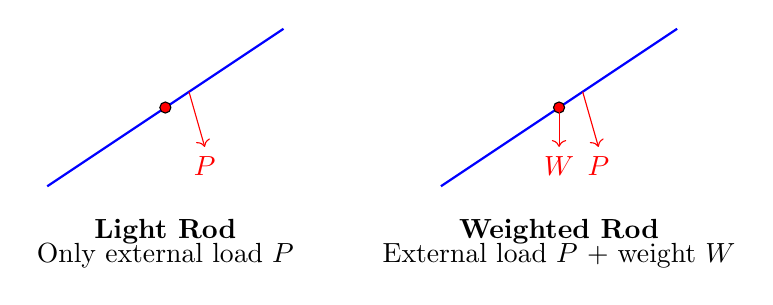
\begin{tikzpicture}[scale=1]
% Light rod
\begin{scope}[xshift=0cm]
\draw[thick, blue] (0,0) -- (3,2);
\draw[fill=red] (1.5,1) circle (2pt);
\draw[red, ->] (1.8,1.2) -- (2,0.5) node[below] {$P$};
\node[below] at (1.5,-0.3) {\textbf{Light Rod}};
\node[below] at (1.5,-0.6) {Only external load $P$};
\end{scope}

% Weighted rod
\begin{scope}[xshift=5cm]
\draw[thick, blue] (0,0) -- (3,2);
\draw[fill=red] (1.5,1) circle (2pt);
\draw[red, ->] (1.5,1) -- (1.5,0.5) node[below] {$W$};
\draw[red, ->] (1.8,1.2) -- (2,0.5) node[below] {$P$};
\node[below] at (1.5,-0.3) {\textbf{Weighted Rod}};
\node[below] at (1.5,-0.6) {External load $P$ + weight $W$};
\end{scope}
\end{tikzpicture}
\end{document}
